\documentclass[10pt, a4paper, fleqn]{article}
\setlength\parindent{0pt}
\usepackage{design_ASC}
\usepackage{amssymb}
\usepackage{array}
\usepackage{varwidth}
\usepackage{cancel}
\usepackage{ulem}
\usepackage{amssymb, amsmath, bm}
\usepackage{subfigure}
\title{Ability of Open-Source VS Closed-Source to Fix Bugs Over Time}
\date{May 17$^{th}$, 2021}
\author{Omri Bornstein | \href{mailto:obor0001@student.monash.edu}{obor0001@student.monash.edu}}
\begin{document}
\maketitle
\section*{Author Contributions}
OB proposed the research question, designed the study, wrangled the data, analysed the results, drafted and edited the paper.
\section{Abstract}
The aim of this project is to simulate both development approaches with agent-based simulations that introduces bug points based on a predefined probability and records the amount of bug points eliminated over time. The rate of bugs eliminated over time of each agent group will be determined by comparing the number of bugs acknowledged and solved by the Linux and Windows development teams. As the simulation unfolds, the total number of bugs fixed over time was recorded, which will be converted into a chart in order to provide a clearer insight into the bug-related implications of using each approach. The insights from this project might assist software developers, technology companies and computer scientists to decide more informatively for themselves which development model is better for their circumstance. Nowadays the comparison between open-source software and closed-source influences global infrastructure (Zemlin 2016), scientific research (Wilson \& Tchantchaleishvili 2013) and how software is maintained and distributed (Volpi 2019).
\section{Keywords}
Open-source, Closed-source, Software bugs, Simulation
\section{Introduction}
Many software-related professionals ask themselves: What software development and distribution model (open-source/closed-source) is better for software stability (based on bug fixes) over time? This study aims to attempt tucking this question by using an agent based simulation in order to model the team dynamics of open-source (O’Neill 2012) development, where the team members are free to collaborate with anyone they wish, and closed-source development, where team members cannot easily collaborate with outsiders. In this paper, the methods of the study (simulation logic, data collection and statistical analysis), the results of the simulation and relevant discussion are featured.
\section{Method}
\subsection{Simulation Logic}
In order to answer the research question mentioned above, I will construct an agent-based simulation with the following agents:
\begin{itemize}
	\item A software bug agent that:
	\begin{itemize}
		\item can spawn randomly for each increment in time
		\item is eliminated after a set number of links by software developer
	\end{itemize}
	\item A software developer agent that:
	\begin{itemize}
		\item is associated with a group
		\item can link to a software bug in order to eliminate it
	\end{itemize}
	\item A group agent that:
	\begin{itemize}
		\item contains a group of software developers
		\item is either be open-source or closed source
		\begin{itemize}
			\item Each group type has a set rate of links its developers can form with bug nodes.
			\item Closed-source groups are only able to operate within their own simulation space.
		\end{itemize}
	\end{itemize}
	The simulation code will keep a record on the timestamp of each bug agent elimination in order to produce a line chart of bug eliminations over time.
\end{itemize}
\begin{figure}[hbt!]
	\centering
	\subfigure[unrestricted collaboration]{\frame{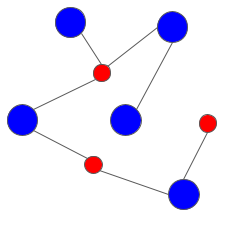
\includegraphics[scale=0.7]{open_env.png}}}
	\subfigure[group-restricted collaboration]{\frame{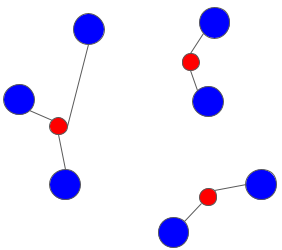
\includegraphics[scale=0.7]{closed_env.png}}}
	\caption{Opposite Environments (left: open, right: closed) With \textcolor{blue}{developer nodes} and \textcolor{red}{bug nodes}}
\end{figure}
\subsection{Data Collection}
The data this simulation is based of was sourced from \href{https://cve.mitre.org/data/downloads/index.html}{MITRE}'s CVE database. Initially, the database CSV file was wrangled manually in order to format the header correctly in order for it work well with Pandas. After that, only CVE records with the substrings of "Linux" or "Windows" were considered. From these CVE's the year of submission was extracted from the CVE ID to be aggregated into a collective number of CVEs for each year and operating system since 1999 to 2020. From the wrangled data, the mean ($\bar{X}$) divided by the total of the number of CVEs for each OS was used as the probability of new bugs being generated and the standard deviation ($\sigma$) divided by the total of the number of CVEs for each OS was used for the probability of a developer node to form an edge to a bug node.
\begin{figure}[hbt!]
	\centering
	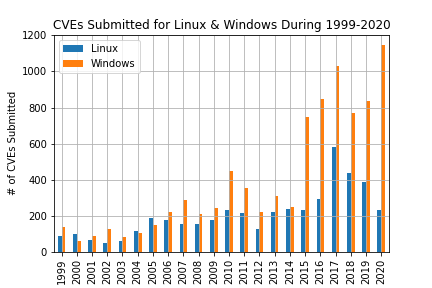
\includegraphics[scale=0.6]{base_data.png}
	\caption{CVEs Submitted for Linux \& Windows During 1999-2020}
\end{figure}
According to MITRE's CVE database, between 1999-2020:
\begin{itemize}
	\item Linux's:
	\begin{itemize}
		\item mean ($\bar{X}$) number of CVE submissions is 205.727273
		\item standard deviation ($\sigma$) for the number of CVE submissions is 128.656124
		\item total number of CVE submission is 4612
	\end{itemize}
	\item Windows's:
	\begin{itemize}
		\item mean ($\bar{X}$) number of CVE submissions is 394.181818
		\item standard deviation ($\sigma$) for the number of CVE submissions is 337.224475
		\item total number of CVE submission is 8931
	\end{itemize}
\end{itemize}
\subsection{Statistical Analysis}
The simulation consistent of 10,000 timestamps and was repeated for 20 times. For each timestamp of the 20 trials, the mean ($\bar{X}$) and standard deviation ($\sigma$) was calculated across all 20 trials.
\section{Results}
As shown in the Figure 2 and Figure 3, both the mean and standard deviation are mostly consistent across all 20 trials. The mean number of removed bug nodes are mostly between 0.1 and 0.15, and the standard deviation is mostly between 0.2 and 0.3.
\bigbreak
It is suspected that due to the current configuration of 25 developer nodes with a maximum of 3 connected bug nodes for each of them, some developer nodes could not connect with bug nodes because there were not left any for them.
\begin{figure}[hbt!]
	\centering
	\subfigure[$\bar{X}$ of Bug Nodes Removed For Each Timestamp]{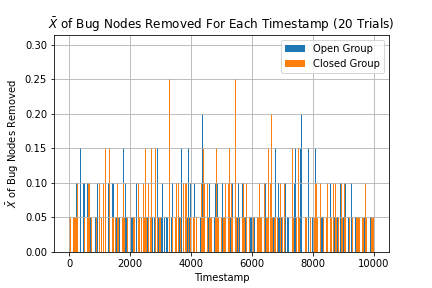
\includegraphics[scale=0.6]{mean.png}}
	\subfigure[$\sigma$ of Bug Nodes Removed For Each Timestamp]{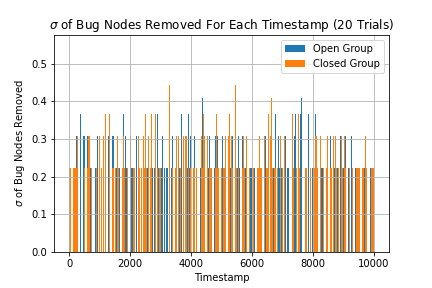
\includegraphics[scale=0.6]{std.png}}
	\caption{$\bar{X}$ \& $\sigma$ of Bug Nodes Removed For Each Timestamp (20 Trials)}
\end{figure}
\section{Discussion}
Due to the mostly consistent and the simulation's logic, the number of bug nodes removed does not vary significantly enough over timestamps in order to reject the null hypothesis. This behavior of the simulation does not mimic reality accurately enough to produce a meaningful outcome. Therefore, a continuation to this study is required to feature a more comprehensive dataset and a more sophisticated agent-based simulation.
\bigbreak
The open-source side of the simulation attempted to mimic the way open-source software is being developed in the real world, which shutters the notion of software as patent by allowing anybody to audit and modify the source code (Fuggetta 2003)(O’Neill 2012). This manifested in the simulation by allowing developer nodes to access any bug node. The closed-source group was composed of two smaller open-source-like groups that can only access bugs generated in their group. It is suspected that current implementation of random bug node generation and elimination does not simulate closely enough the way closed-source software teams operate in the real world.
\section{Conclusion}
In conclusion, the basic logic and architecture for this study's simulation are established, but they are not comprehensive enough to mimic the real world. Future research into this field should use more comprehensive data that would allow the simulation to randomly generate and eliminate bug nodes in a more complex manner.
\newpage\section{Bibliography}
\begin{itemize}
	\item Bonaccorsi, Andrea, and Cristina Rossi. 2003. "Why Open Source Software Can Succeed." Research Policy 32 (7): 1243–58. \url{https://doi.org/10.1016/s0048-7333(03)00051-9}.
	\item Brigham, Katie, Lindsey Jacobson, and CNBC. 2019. "The Rise of Open-Source Software." YouTube Video. CNBC. \url{https://youtu.be/SpeDK1TPbew}.
	\item Dhir, Swati, and Sanjay Dhir. 2017. "Adoption of Open-Source Software versus Proprietary Software: An Exploratory Study." Strategic Change 26 (4): 363–71. \url{https://doi.org/10.1002/jsc.2137}.
	\item Fioretti, Guido. 2012. "Agent-Based Simulation Models in Organization Science." Organizational Research Methods 16 (2): 227–42. \url{https://doi.org/10.1177/1094428112470006}.
	\item Fuggetta, Alfonso. 2003. "Open Source Software––an Evaluation." Journal of Systems and Software 66 (1): 77–90. \url{https://doi.org/10.1016/s0164-1212(02)00065-1}.
	\item Gambardella, Alfonso, and Bronwyn H. Hall. 2006. "Proprietary versus Public Domain Licensing of Software and Research Products." Research Policy 35 (6): 875–92. \url{https://doi.org/10.1016/j.respol.2006.04.004}.
	\item Kahl, Cara H., and Matthias Meyer. 2016. "Constructing Agent-Based Models of Organizational Routines." In Agent-Based Simulation of Organizational Behavior, edited by Davide Secchi and Martin Neumann, 1st ed., 85–107. Switzerland: Cham Springer International Publishing. \url{https://doi.org/10.1007/978-3-319-18153-0\_5}.
	\item Lanzi, Diego. 2009. "Competition and Open Source with Perfect Software Compatibility." Information Economics and Policy 21 (3): 192–200. \url{https://doi.org/10.1016/j.infoecopol.2008.11.004}.
	\item MITRE Corporation. 2021. "CVE - Download CVE List." Mitre.org. January 5, 2021. \url{https://cve.mitre.org/data/downloads/index.html}.
	\item Murray, Dale. 2020. "Open Source and Security: Why Transparency Now Equals Strength." Network Security 2020 (7): 17–19. \url{https://doi.org/10.1016/s1353-4858(20)30082-9}.
	\item Nagy, Del, Areej M. Yassin, and Anol Bhattacherjee. 2010. "Organizational Adoption of Open Source Software." Communications of the ACM 53 (3): 148–51. \url{https://doi.org/10.1145/1666420.1666457}.
	\item O’Neill, Allen. 2012. "Open Source Software." In Encyclopedia of Applied Ethics, 2nd ed., 281–87. Elsevier. \url{https://doi.org/10.1016/b978-0-12-373932-2.00063-6}.
	\item Välimäki, Mikko, and Ville Oksanen. 2005. "The Impact of Free and Open Source Licensing on Operating System Software Markets." Telematics and Informatics 22 (1-2): 97–110. \url{https://doi.org/10.1016/j.tele.2004.06.008}.
	\item Volpi, Mike. 2019. "How Open-Source Software Took over the World." TechCrunch. TechCrunch. January 12, 2019. \url{https://techcrunch.com/2019/01/12/how-open-source-software-took-over-the-world/}.
	\item Zemlin, Jim. 2016. "What the Tech Industry Has Learned from Linus Torvalds." YouTube Video. TEDx Talks. \url{https://youtu.be/7XTHdcmjenI}.
\end{itemize}
\end{document}